\documentclass[UTF8,12pt,a4paper]{ctexart}

\usepackage{amsmath}
\usepackage{cases}
\usepackage{cite}
\usepackage{graphicx}
\usepackage{enumerate}
\usepackage{algorithm}
\usepackage{caption}   % \caption*需要
\usepackage{subcaption} % 子图布局
\usepackage[noend]{algpseudocode} %algorithmicx
\makeatletter
\renewcommand{\fnum@algorithm}{\fname@algorithm}
\makeatother
\renewcommand{\algorithmicrequire}{\textbf{Input:}}
\renewcommand{\algorithmicensure}{\textbf{Output:}}
\usepackage[margin=1in]{geometry}
\geometry{a4paper}
\usepackage{fancyhdr}
\pagestyle{fancy}
\fancyhf{}
\usepackage{xcolor}





% ------------------- 设置超链接，便于跳转 -----------------
\usepackage{enumitem}
\usepackage{hyperref}
\hypersetup{
    pdfborder={0 0 0},    % 消除超链接边框
    colorlinks=true,       % 将边框改为颜色标记（可选）
    linkcolor=black,       % 内部链接颜色（目录、引用等）
    citecolor=black,       % 引用颜色
    urlcolor=blue          % URL链接颜色（保持蓝色以便区分）
}



% ------------------------ 标题区 ----------------------------
\title{AIC Lab2 实验报告}
\author{
	姓名：\underline{冯峻}~~~~~~
	学号：\underline{523031910148}~~~~~~}
\date{\today}
\pagenumbering{arabic}

\begin{document}



% ------------------------ 页眉和页脚 ----------------------------
\fancyhead[L]{冯峻}
\fancyhead[C]{AIC Lab2}
\fancyfoot[C]{\thepage}

\maketitle
\tableofcontents
\newpage

\section{任务一：电流镜}

\subsection{实验电路}
任务一主要电路图见图\ref{fig:current_mirror_circuit}所示。

我们有：
\begin{equation}
V_{\text{GS4}} = V_{\text{GS3}} - I_{\text{out}}R_{\text{S}}
\end{equation}
假设电流镜中的各个晶体管工作在饱和区，因此有：
\begin{equation}
\sqrt{\frac{2I_{\text{out}}}{\mu_{\text{p}} C_{\text{ox}} (W/L)_{\text{P}}}} + V_{\text{THP}4} = \sqrt{\frac{2I_{\text{out}}}{\mu_{\text{p}} C_{\text{ox}} K(W/L)_{\text{P}}}} + V_{\text{THP}3} - I_{\text{out}}R_{\text{S}}
\end{equation}
因此有：
\begin{equation}
I_{\text{out}} = \frac{2}{\mu_{\text{p}} C_{\text{ox}} (W/L)_{\text{P}}}\frac{1}{R_{\text{S}}^2}(\frac{1}{\sqrt{K}}-1)^2
\end{equation}
\begin{figure}[h]
    \centering
    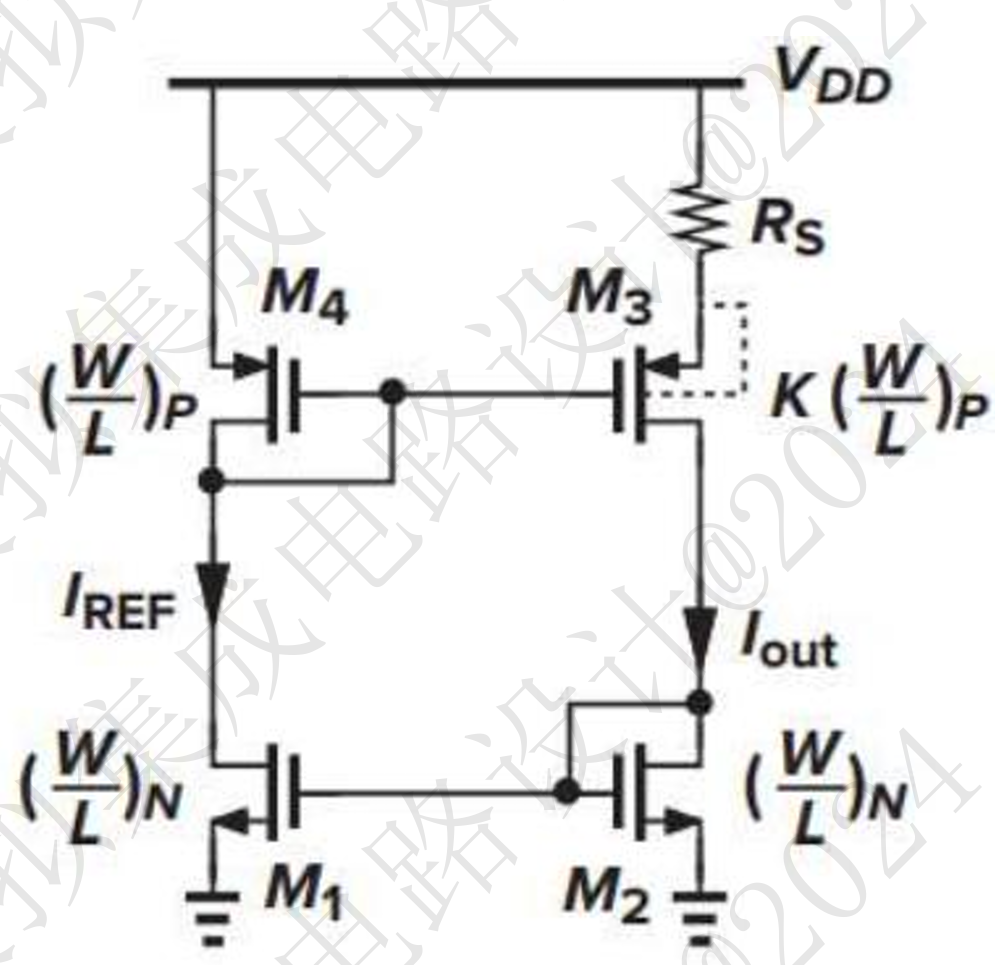
\includegraphics[width=0.7\textwidth]{Fig/电流镜电路图.png}
    \caption{电流镜实验电路图}
    \label{fig:current_mirror_circuit}
\end{figure}
\subsection{任务1.1}
\textbf{任务内容：参考书本结合DC工作点计算和电流仿真结果，分析两者是否吻合}

直流工作点仿真结果如图\ref{fig:task1_1_dc}所示：

\begin{figure}[h]
\centering

\includegraphics[width=0.7\textwidth]{Fig/image.png}
\caption{电流镜直流工作点仿真}
\label{fig:task1_1_dc}
\end{figure}

各晶体管的关键电压和电流参数如表\ref{tab:task1_1}所示：

\begin{table}[h]
\centering
\caption{电流镜各晶体管DC工作点参数}
\label{tab:task1_1}
\begin{tabular}{|c|c|c|c|c|c|c|}
\hline
MOSFET & $V_{GS}$/mV & $V_{DS}$/mV & $I_{DS}$/$\mu$A & $V_{\text{TH}}$/mV & $V_{\text{DSAT}}$/mV & region\\
\hline
M1 & 547.795 & 535.389 & 9.807 & 367.632 & 105.3  & 2\\
\hline
M2 & 547.785 & 547.795 & 9.836 & 367.606 & 105.312  & 2\\
\hline
M3 & -507.241 & -494.835 & -9.836 & -456.654 & -107.887  & 2\\
\hline
M4 & -664.611 & -664.611 & -9.807 & -456.524 & -227.131 & 2\\
\hline
\end{tabular}
\end{table}

\textbf{理论分析：}
从表\ref{tab:task1_1}可以看出，所有晶体管均工作在饱和区(region=2)，符合电流镜的设计要求。
此部分理论分析待完善。

\subsection{任务1.2}
\textbf{任务内容：通过DC仿真，设置$V_{\text{DD}}$为变化量，得出$V_{\text{DD}}$与电流的关系，并绘图}

通过DC仿真，设置$V_{\text{DD}}$为扫描变量，得到$I_{\text{out}} - V_{\text{DD}}$曲线如图\ref{fig:task1_2}所示：

\begin{figure}[htbp]
    \centering
    % 第一张子图
    \begin{subfigure}[b]{0.45\textwidth} % 子图宽度为总宽度的45%
        \centering
        
\includegraphics[width=\textwidth]{Fig/image-9.png}
        \caption{$I_{\text{out}} - V_{\text{DD}}$关系曲线}
        \label{fig:task1_2}
    \end{subfigure}
    \hfill % 添加水平间距
    % 第二张子图
    \begin{subfigure}[b]{0.45\textwidth}
        \centering
        
\includegraphics[width=\textwidth]{Fig/image-8.png}
        \caption{$I_{\text{out}} - T$关系曲线}
        \label{fig:task1_3}
    \end{subfigure}
    % 总图标题
    \caption{电流镜特性曲线}
    \label{fig:current_mirror_characteristics}
\end{figure}

从仿真结果可以观察到，当$V_{\text{DD}}$从0V变化到1.2V时，输出电流$I_{\text{out}}$逐渐增大。分析待补充

\subsection{任务1.3}
\textbf{任务内容：通过DC仿真，设置温度为变化量（温度仿真设置0℃-70℃），得出温度与电流的关系，并绘图。温度扫描方法见第三部分}

通过DC仿真，设置温度为扫描变量（温度范围0℃-70℃），得到$I_{\text{out}} - T$曲线如图\ref{fig:task1_3}所示：

从仿真结果可以看出，输出电流随温度的上升呈线性上升。分析待补充

\subsection{任务1.4}
\textbf{任务内容：设置工艺角（TT/FF/SS）重复2/3，并绘图。Corner设置方法见第四部分）}

在不同工艺角（TT/FF/SS）下进行DC仿真，得到电流-$V_{\text{DD}}$曲线如图\ref{fig:task1_4_vdd}所示以及电流-温度曲线如图\ref{fig:task1_4_temp}所示：

\begin{figure}[htbp]
    \centering
    % 第一张子图
    \begin{subfigure}[b]{0.45\textwidth} % 子图宽度为总宽度的45%
        \centering
        
\includegraphics[width=0.8\textwidth]{Fig/image-4.png}
        \caption{不同工艺角下的$I_{\text{out}} - V_{\text{DD}}$曲线}
        \label{fig:task1_4_vdd}
    \end{subfigure}
    \hfill % 添加水平间距
    % 第二张子图
    \begin{subfigure}[b]{0.45\textwidth}
        \centering
        
\includegraphics[width=\textwidth]{Fig/image-5.png}
        \caption{不同工艺角下的$I_{\text{out}} - T$曲线}
        \label{fig:task1_4_temp}
    \end{subfigure}
    % 总图标题
    \caption{不同工艺角下的电流特性曲线}
    \label{fig:corner}
\end{figure}


从图\ref{fig:task1_4_vdd}可以发现，当$V_{\text{DD}}<0.9V$时，ff工艺角的$I_{\text{out}}$最大，ss工艺角的$I_{\text{out}}$最小。当$V_{\text{DD}} > 0.9V$时，ff工艺角的$I_{\text{out}}$最小，tt工艺角和ss工艺角的$I_{\text{out}}$几乎相同。

从图\ref{fig:task1_4_temp}可以发现，三种工艺角下，$I_{\text{out}}$均随着温度上升而呈线性上升。

\subsection{任务1.5}
\textbf{任务内容：基于以上结果，简要分析温度、电压和工艺对电流的影响}


\newpage
\section{任务二：差分对}

\subsection{实验电路}
任务二主要电路图见图\ref{fig:diff_pair_circuit}所示。
\begin{figure}[h]
    \centering
    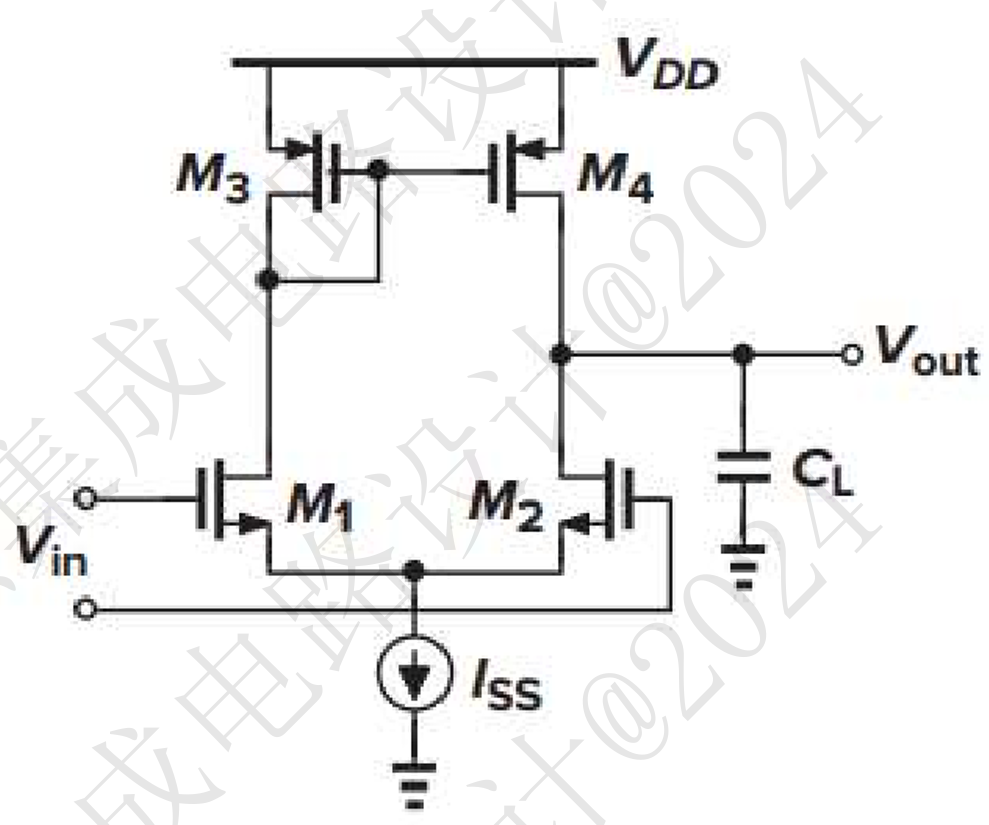
\includegraphics[width=0.7\textwidth]{Fig/差分对电路图.png}
    \caption{差分对实验电路图}
    \label{fig:diff_pair_circuit}
\end{figure}
\subsection{任务2.1}
\textbf{任务内容：采用1中的电流源，利用基本电流镜复制，替换ISS}

设计的差分放大器顶层电路测试图如图\ref{fig:task2_1_top}所示;
电流镜原理图（即任务一中的电流镜）如图\ref{fig:task2_1_mirror}所示;
差分对原理图如图\ref{fig:task2_1_diff}所示；
差分信号生成电路图如图\ref{fig:task2_1_signal}所示。

提供电流源$I_{\text{SS}}$的方法是：提取任务一中电流镜电路的NMOS栅极电位，并将其作为偏置电压$V_{\text{b}}$连接到差分对电路中作为NMOS的栅极电位，从而使得该NMOS称为一个电流源。

\begin{figure}[htbp]
    \centering
    % 第一张子图
    \begin{subfigure}[b]{0.45\textwidth} % 子图宽度为总宽度的45%
        \centering
        
\includegraphics[width=\textwidth]{Fig/image-10.png}
        \caption{差分放大器顶层电路测试图}
        \label{fig:task2_1_top}
    \end{subfigure}
    \hfill % 添加水平间距
    % 第二张子图
    \begin{subfigure}[b]{0.45\textwidth}
        \centering
        
\includegraphics[width=\textwidth]{Fig/image-11.png}
        \caption{电流镜原理图}
        \label{fig:task2_1_mirror}
    \end{subfigure}
    % 总图标题
    \caption{差分对电路图1}
    \label{fig:差分对电路图1}
\end{figure}

\begin{figure}[htbp]
    \centering
    % 第一张子图
    \begin{subfigure}[b]{0.45\textwidth} % 子图宽度为总宽度的45%
        \centering
        
\includegraphics[width=\textwidth]{Fig/image-12.png}
        \caption{差分对原理图}
        \label{fig:task2_1_diff}
    \end{subfigure}
    \hfill % 添加水平间距
    % 第二张子图
    \begin{subfigure}[b]{0.45\textwidth}
        \centering
        
\includegraphics[width=\textwidth]{Fig/image-16.png}
        \caption{差分信号生成电路图}
        \label{fig:task2_1_signal}
    \end{subfigure}
    % 总图标题
    \caption{差分对电路图2}
    \label{fig:差分对电路图2}
\end{figure}





\subsection{任务2.2}
\textbf{任务内容：M1/M2设置为100um/100nm，M3/M4设置为8um/1um，CL为1pF。进行直流仿真，分析所有晶体管的工作区间}

电流镜直流工作点仿真图像如图\ref{fig:task2_2_mirror_dc}所示：

\begin{figure}[htbp]
    \centering
    % 第一张子图
    \begin{subfigure}[b]{0.45\textwidth} % 子图宽度为总宽度的45%
        \centering
        
\includegraphics[width=\textwidth]{Fig/image-6.png}
        \caption{电流镜直流工作点仿真}
        \label{fig:task2_2_mirror_dc}
    \end{subfigure}
    \hfill % 添加水平间距
    % 第二张子图
    \begin{subfigure}[b]{0.45\textwidth}
        \centering
        
\includegraphics[width=\textwidth]{Fig/image-7.png}
        \caption{差分对直流工作点仿真}
        \label{fig:task2_2_diff_dc}
    \end{subfigure}
    % 总图标题
    \caption{差分对电路直流工作点}
    \label{fig:差分对电路直流工作点}
\end{figure}


电流镜中所有晶体管的直流工作点如表\ref{tab:task2_2_mirror}所示：

\begin{table}[h]
\centering
\caption{电流镜各晶体管DC工作点参数}
\label{tab:task2_2_mirror}
\begin{tabular}{|c|c|c|c|c|c|}
\hline
MOSFET & $V_{GS}$/mV & $V_{DS}$/mV & $I_{DS}$/$\mu$A & $V_{\text{TH}}$/mV & $V_{\text{DSAT}}$/mV \\
\hline
M1 & 547.794 & 535.39 & 9.807 & 367.632 & 105.299 \\
\hline
M2 & 547.794 & 547.794 & 9.836 & 367.606 & 105.312 \\
\hline
M3 & -507.241 & -494.836 & -9.836 & -456.654 & -107.887 \\
\hline
M4 & -664.61 & -664.61 & -9.807 & -456.524 & -227.13 \\
\hline
\end{tabular}
\end{table}

\textbf{电流镜晶体管工作区间分析：}

\begin{itemize}
\item \textbf{M1（NMOS）：}$V_{GS} = 547.794\text{mV} > V_{TH} = 367.632\text{mV}$，晶体管导通；$V_{DS} = 535.39\text{mV} > V_{DSAT} = 105.299\text{mV}$，因此M1工作在\textbf{饱和区}。

\item \textbf{M2（NMOS）：}$V_{GS} = 547.794\text{mV} > V_{TH} = 367.606\text{mV}$，晶体管导通；$V_{DS} = 547.794\text{mV} > V_{DSAT} = 105.312\text{mV}$，因此M2工作在\textbf{饱和区}。

\item \textbf{M3（PMOS）：}$|V_{GS}| = 507.241\text{mV} > |V_{TH}| = 456.654\text{mV}$，晶体管导通；$|V_{DS}| = 494.836\text{mV} > |V_{DSAT}| = 107.887\text{mV}$，因此M3工作在\textbf{饱和区}。

\item \textbf{M4（PMOS）：}$|V_{GS}| = 664.61\text{mV} > |V_{TH}| = 456.524\text{mV}$，晶体管导通；$|V_{DS}| = 664.61\text{mV} > |V_{DSAT}| = 227.13\text{mV}$，因此M4工作在\textbf{饱和区}。
\end{itemize}

差分对直流工作点仿真图像如图\ref{fig:task2_2_diff_dc}所示。

差分对中所有晶体管的直流工作点如表\ref{tab:task2_2_diff}所示：

\begin{table}[h]
\centering
\caption{差分对各晶体管DC工作点参数}
\label{tab:task2_2_diff}
\begin{tabular}{|c|c|c|c|c|c|}
\hline
MOSFET & $V_{GS}$/mV & $V_{DS}$/mV & $I_{DS}$/$\mu$A & $V_{\text{TH}}$/mV & $V_{\text{DSAT}}$/mV \\
\hline
M1 & 278.599 & 365.873 & 4.599 & 384.56 & 41.5285 \\
\hline
M2 & 278.599 & 365.873 & 4.599 & 384.56 & 41.5285 \\
\hline
M3 & -512.726 & -512.726 & -4.599 & -403.135 & -120.446 \\
\hline
M4 & -512.726 & -512.726 & -4.599 & -403.135 & -120.446 \\
\hline
$M_{\text{SS}}$ & 547.794 & 321.401 & 9.197 & 368.08 & 105.086 \\
\hline
\end{tabular}
\end{table}

\textbf{差分对晶体管工作区间分析：}

\begin{itemize}
\item \textbf{M1（NMOS）：}$V_{GS} = 278.599\text{mV} < V_{TH} = 384.56\text{mV}$，因此M1工作在\textbf{截止区}。

\item \textbf{M2（NMOS）：}$V_{GS} = 278.599\text{mV} < V_{TH} = 384.56\text{mV}$，因此M2工作在\textbf{截止区}。

\item \textbf{M3（PMOS）：}$|V_{GS}| = 512.726\text{mV} > |V_{TH}| = 403.135\text{mV}$，晶体管导通；$|V_{DS}| = 512.726\text{mV} > |V_{DSAT}| = 120.446\text{mV}$，因此M3工作在\textbf{饱和区}。

\item \textbf{M4（PMOS）：}$|V_{GS}| = 512.726\text{mV} > |V_{TH}| = 403.135\text{mV}$，晶体管导通；$|V_{DS}| = 512.726\text{mV} > |V_{DSAT}| = 120.446\text{mV}$，因此M4工作在\textbf{饱和区}。

\item \textbf{$M_{\text{SS}}$（NMOS）：}$V_{GS} = 547.794\text{mV} > V_{TH} = 368.08\text{mV}$，晶体管导通；$V_{DS} = 321.401\text{mV} > V_{DSAT} = 105.086\text{mV}$，因此$M_{\text{SS}}$工作在\textbf{饱和区}。
\end{itemize}

\subsection{任务2.3}
\textbf{任务内容：扫描M3/M4的宽度，将Vout的静态工作点设置为0.6V，记录晶体管设计参数和结果}

设置$W$从$1\mu\text{m}$扫描至$16\mu\text{m}$，进行DC仿真，得到$V_{\text{out}}$直流工作点电压与$W$的关系图如图\ref{fig:task2_3_1}和图\ref{fig:task2_3_2}所示：


\begin{figure}[htbp]
    \centering
    % 第一张子图
    \begin{subfigure}[b]{0.45\textwidth} % 子图宽度为总宽度的45%
        \centering
        
\includegraphics[width=\textwidth]{Fig/image-14.png}
        \caption{$V_{\text{out}} - W$关系曲线（图1）}
        \label{fig:task2_3_1}
    \end{subfigure}
    \hfill % 添加水平间距
    % 第二张子图
    \begin{subfigure}[b]{0.45\textwidth}
        \centering
        
\includegraphics[width=\textwidth]{Fig/image-13.png}
        \caption{$V_{\text{out}} - W$关系曲线（图2）}
        \label{fig:task2_3_2}
    \end{subfigure}
    % 总图标题
    \caption{$V_{\text{out}}$直流工作点电压与$W$的关系曲线}
    \label{fig:task2_3}
\end{figure}



从仿真结果可知，当$V_{\text{out}} \approx 600\text{mV}$时，$W\approx 3\mu\text{m}$。因此，为了使输出静态工作点为0.6V，M3和M4的宽度应设计为$3\mu\text{m}$。

\subsection{任务2.4}
\textbf{任务内容：进行小信号AC仿真，结合实验1中的gmro参数和增益公式，对比仿真结果和解析结果，分析低频增益、带宽、增益带宽积}

使用任务2.3中得到的晶体管M3和M4的参数$W=3\mu\text{m}$，进行AC仿真，设置频率从1Hz扫描到1GHz，得到$v_{\text{out}}$的增益与频率的曲线图如图\ref{fig:task2_4}所示：

\begin{figure}[h]
\centering
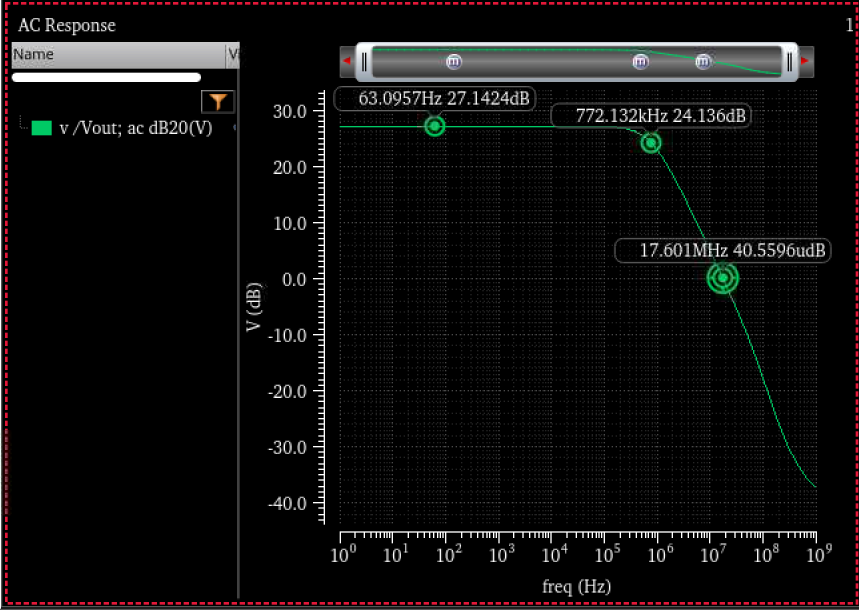
\includegraphics[width=0.8\textwidth]{Fig/增益曲线.png}
\caption{增益-频率特性曲线}
\label{fig:task2_4}
\end{figure}

从仿真结果可以观察到：

\begin{itemize}
\item \textbf{低频增益：}低频增益为27.1424dB。

\item \textbf{带宽：}当$f = 772\text{kHz}$时，增益开始出现明显下降，因此该差分放大器的带宽为$772\text{kHz}$。

\item \textbf{增益带宽积：}当频率来到$f = 17.6\text{MHz}$时，增益下降至0dB。

\end{itemize}

\textbf{理论分析：}

根据教材，五管OTA电路的低频增益公式为：
\begin{equation}
\frac{v_{\text{out}}}{v_{\text{in}}} = g_\text{m1}(r_{\text{ds1} // \text{ds4}})\frac{2g_{\text{m4}}r_{\text{ds4} + 1}}{2(g_{\text{m4}}r_{\text{ds4}}+1)}
\end{equation}
实验测得，直流工作点下，晶体管M1和M4的跨到和输出电阻见图\ref{fig:task2_4_M}所示。

在输出结点$V_{\text{out}}$向上看的电阻为：$r_{\text{ds4}}$，向下看的电阻为：$r_{\text{ds2}}$，负载电容为$C_{\text{L}}$，因此时间常数为：$r_{\text{ds2}}//r_{\text{ds4}}C_{\text{L}}$，我们假设电路中其他寄生电容较小，则主极点频率为：$\frac{1}{2\pi r_{\text{ds2}}//r_{\text{ds4}}C_{\text{L}}}$。

\begin{figure}[htbp]
    \centering
    % 第一张子图
    \begin{subfigure}[b]{0.45\textwidth} % 子图宽度为总宽度的45%
        \centering
        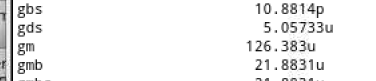
\includegraphics[width=\textwidth]{Fig/M1直流工作参数.png}
        \caption{M1的跨导及输出电阻}
        \label{fig:task2_4_1}
    \end{subfigure}
    \hfill % 添加水平间距
    % 第二张子图
    \begin{subfigure}[b]{0.45\textwidth}
        \centering
        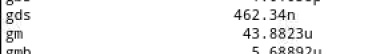
\includegraphics[width=\textwidth]{Fig/M4直流工作参数.png}
        \caption{M4的跨导及输出电阻}
        \label{fig:task2_4_2}
    \end{subfigure}
    % 总图标题
    \caption{M1和M4的直流工作参数}
    \label{fig:task2_4_M}
\end{figure}
可知，$$g_{\text{m1}} = 126.383\text{uS}, g_{\text{ds1}} = 5.057\text{uS}, g_{\text{m4}} = 43.882\text{uS}, g_{\text{ds4}} = 462.3\text{nS}$$ 

因此：
\begin{itemize}
    \item \textbf{低频增益}
    
    $$A_0 = \frac{v_{\text{out}}}{v_{\text{in}}} \approx 22.77 \rightarrow 20\text{lg}\frac{v_{\text{out}}}{v_{\text{in}}} \approx 27.15\text{dB}$$而仿真结果为$27.1424\text{dB}$，
    两者较为接近。证明了理论分析的正确性。

    \item \textbf{带宽}
    
    通过直流工作点仿真可以得到
    $$g_{\text{ds2}} = 4.47\text{uS}$$
    ,求解得到主极点频率为：
    $$f_{\text{p}} = \frac{1}{2\pi r_{\text{ds2}}//r_{\text{ds4}}C_{\text{L}}} \approx 785\text{kHz}$$
    ,而仿真测量出的值为$772\text{kHz}$，两者较为接近。证明了理论分析的正确性。

    \item \textbf{增益带宽积}
    
    增益带宽积的理论值为：
    $$\text{GBW} = \text{BW} \times A_{0} = f_{\text{p}} \times A_{0} = 785\text{kHz} \times 22.77 \approx 17.87\text{MHz}$$
    ，而仿真结果为$17.6\text{MHz}$，两者较为接近。证明了理论分析的正确性。
\end{itemize}

\end{document}
